% Options for packages loaded elsewhere
\PassOptionsToPackage{unicode}{hyperref}
\PassOptionsToPackage{hyphens}{url}
\PassOptionsToPackage{dvipsnames,svgnames,x11names}{xcolor}
%
\documentclass[
  letterpaper,
  DIV=11,
  numbers=noendperiod]{scrartcl}

\usepackage{amsmath,amssymb}
\usepackage{lmodern}
\usepackage{iftex}
\ifPDFTeX
  \usepackage[T1]{fontenc}
  \usepackage[utf8]{inputenc}
  \usepackage{textcomp} % provide euro and other symbols
\else % if luatex or xetex
  \usepackage{unicode-math}
  \defaultfontfeatures{Scale=MatchLowercase}
  \defaultfontfeatures[\rmfamily]{Ligatures=TeX,Scale=1}
\fi
% Use upquote if available, for straight quotes in verbatim environments
\IfFileExists{upquote.sty}{\usepackage{upquote}}{}
\IfFileExists{microtype.sty}{% use microtype if available
  \usepackage[]{microtype}
  \UseMicrotypeSet[protrusion]{basicmath} % disable protrusion for tt fonts
}{}
\makeatletter
\@ifundefined{KOMAClassName}{% if non-KOMA class
  \IfFileExists{parskip.sty}{%
    \usepackage{parskip}
  }{% else
    \setlength{\parindent}{0pt}
    \setlength{\parskip}{6pt plus 2pt minus 1pt}}
}{% if KOMA class
  \KOMAoptions{parskip=half}}
\makeatother
\usepackage{xcolor}
\setlength{\emergencystretch}{3em} % prevent overfull lines
\setcounter{secnumdepth}{-\maxdimen} % remove section numbering
% Make \paragraph and \subparagraph free-standing
\ifx\paragraph\undefined\else
  \let\oldparagraph\paragraph
  \renewcommand{\paragraph}[1]{\oldparagraph{#1}\mbox{}}
\fi
\ifx\subparagraph\undefined\else
  \let\oldsubparagraph\subparagraph
  \renewcommand{\subparagraph}[1]{\oldsubparagraph{#1}\mbox{}}
\fi

\usepackage{color}
\usepackage{fancyvrb}
\newcommand{\VerbBar}{|}
\newcommand{\VERB}{\Verb[commandchars=\\\{\}]}
\DefineVerbatimEnvironment{Highlighting}{Verbatim}{commandchars=\\\{\}}
% Add ',fontsize=\small' for more characters per line
\usepackage{framed}
\definecolor{shadecolor}{RGB}{241,243,245}
\newenvironment{Shaded}{\begin{snugshade}}{\end{snugshade}}
\newcommand{\AlertTok}[1]{\textcolor[rgb]{0.68,0.00,0.00}{#1}}
\newcommand{\AnnotationTok}[1]{\textcolor[rgb]{0.37,0.37,0.37}{#1}}
\newcommand{\AttributeTok}[1]{\textcolor[rgb]{0.40,0.45,0.13}{#1}}
\newcommand{\BaseNTok}[1]{\textcolor[rgb]{0.68,0.00,0.00}{#1}}
\newcommand{\BuiltInTok}[1]{\textcolor[rgb]{0.00,0.23,0.31}{#1}}
\newcommand{\CharTok}[1]{\textcolor[rgb]{0.13,0.47,0.30}{#1}}
\newcommand{\CommentTok}[1]{\textcolor[rgb]{0.37,0.37,0.37}{#1}}
\newcommand{\CommentVarTok}[1]{\textcolor[rgb]{0.37,0.37,0.37}{\textit{#1}}}
\newcommand{\ConstantTok}[1]{\textcolor[rgb]{0.56,0.35,0.01}{#1}}
\newcommand{\ControlFlowTok}[1]{\textcolor[rgb]{0.00,0.23,0.31}{#1}}
\newcommand{\DataTypeTok}[1]{\textcolor[rgb]{0.68,0.00,0.00}{#1}}
\newcommand{\DecValTok}[1]{\textcolor[rgb]{0.68,0.00,0.00}{#1}}
\newcommand{\DocumentationTok}[1]{\textcolor[rgb]{0.37,0.37,0.37}{\textit{#1}}}
\newcommand{\ErrorTok}[1]{\textcolor[rgb]{0.68,0.00,0.00}{#1}}
\newcommand{\ExtensionTok}[1]{\textcolor[rgb]{0.00,0.23,0.31}{#1}}
\newcommand{\FloatTok}[1]{\textcolor[rgb]{0.68,0.00,0.00}{#1}}
\newcommand{\FunctionTok}[1]{\textcolor[rgb]{0.28,0.35,0.67}{#1}}
\newcommand{\ImportTok}[1]{\textcolor[rgb]{0.00,0.46,0.62}{#1}}
\newcommand{\InformationTok}[1]{\textcolor[rgb]{0.37,0.37,0.37}{#1}}
\newcommand{\KeywordTok}[1]{\textcolor[rgb]{0.00,0.23,0.31}{#1}}
\newcommand{\NormalTok}[1]{\textcolor[rgb]{0.00,0.23,0.31}{#1}}
\newcommand{\OperatorTok}[1]{\textcolor[rgb]{0.37,0.37,0.37}{#1}}
\newcommand{\OtherTok}[1]{\textcolor[rgb]{0.00,0.23,0.31}{#1}}
\newcommand{\PreprocessorTok}[1]{\textcolor[rgb]{0.68,0.00,0.00}{#1}}
\newcommand{\RegionMarkerTok}[1]{\textcolor[rgb]{0.00,0.23,0.31}{#1}}
\newcommand{\SpecialCharTok}[1]{\textcolor[rgb]{0.37,0.37,0.37}{#1}}
\newcommand{\SpecialStringTok}[1]{\textcolor[rgb]{0.13,0.47,0.30}{#1}}
\newcommand{\StringTok}[1]{\textcolor[rgb]{0.13,0.47,0.30}{#1}}
\newcommand{\VariableTok}[1]{\textcolor[rgb]{0.07,0.07,0.07}{#1}}
\newcommand{\VerbatimStringTok}[1]{\textcolor[rgb]{0.13,0.47,0.30}{#1}}
\newcommand{\WarningTok}[1]{\textcolor[rgb]{0.37,0.37,0.37}{\textit{#1}}}

\providecommand{\tightlist}{%
  \setlength{\itemsep}{0pt}\setlength{\parskip}{0pt}}\usepackage{longtable,booktabs,array}
\usepackage{calc} % for calculating minipage widths
% Correct order of tables after \paragraph or \subparagraph
\usepackage{etoolbox}
\makeatletter
\patchcmd\longtable{\par}{\if@noskipsec\mbox{}\fi\par}{}{}
\makeatother
% Allow footnotes in longtable head/foot
\IfFileExists{footnotehyper.sty}{\usepackage{footnotehyper}}{\usepackage{footnote}}
\makesavenoteenv{longtable}
\usepackage{graphicx}
\makeatletter
\def\maxwidth{\ifdim\Gin@nat@width>\linewidth\linewidth\else\Gin@nat@width\fi}
\def\maxheight{\ifdim\Gin@nat@height>\textheight\textheight\else\Gin@nat@height\fi}
\makeatother
% Scale images if necessary, so that they will not overflow the page
% margins by default, and it is still possible to overwrite the defaults
% using explicit options in \includegraphics[width, height, ...]{}
\setkeys{Gin}{width=\maxwidth,height=\maxheight,keepaspectratio}
% Set default figure placement to htbp
\makeatletter
\def\fps@figure{htbp}
\makeatother

\KOMAoption{captions}{tableheading}
\makeatletter
\makeatother
\makeatletter
\makeatother
\makeatletter
\@ifpackageloaded{caption}{}{\usepackage{caption}}
\AtBeginDocument{%
\ifdefined\contentsname
  \renewcommand*\contentsname{Table of contents}
\else
  \newcommand\contentsname{Table of contents}
\fi
\ifdefined\listfigurename
  \renewcommand*\listfigurename{List of Figures}
\else
  \newcommand\listfigurename{List of Figures}
\fi
\ifdefined\listtablename
  \renewcommand*\listtablename{List of Tables}
\else
  \newcommand\listtablename{List of Tables}
\fi
\ifdefined\figurename
  \renewcommand*\figurename{Figure}
\else
  \newcommand\figurename{Figure}
\fi
\ifdefined\tablename
  \renewcommand*\tablename{Table}
\else
  \newcommand\tablename{Table}
\fi
}
\@ifpackageloaded{float}{}{\usepackage{float}}
\floatstyle{ruled}
\@ifundefined{c@chapter}{\newfloat{codelisting}{h}{lop}}{\newfloat{codelisting}{h}{lop}[chapter]}
\floatname{codelisting}{Listing}
\newcommand*\listoflistings{\listof{codelisting}{List of Listings}}
\makeatother
\makeatletter
\@ifpackageloaded{caption}{}{\usepackage{caption}}
\@ifpackageloaded{subcaption}{}{\usepackage{subcaption}}
\makeatother
\makeatletter
\@ifpackageloaded{tcolorbox}{}{\usepackage[many]{tcolorbox}}
\makeatother
\makeatletter
\@ifundefined{shadecolor}{\definecolor{shadecolor}{rgb}{.97, .97, .97}}
\makeatother
\makeatletter
\makeatother
\ifLuaTeX
  \usepackage{selnolig}  % disable illegal ligatures
\fi
\IfFileExists{bookmark.sty}{\usepackage{bookmark}}{\usepackage{hyperref}}
\IfFileExists{xurl.sty}{\usepackage{xurl}}{} % add URL line breaks if available
\urlstyle{same} % disable monospaced font for URLs
\hypersetup{
  pdftitle={Quarto Assignment 1},
  pdfauthor={Anjolaoluwa Olatunbosun},
  colorlinks=true,
  linkcolor={blue},
  filecolor={Maroon},
  citecolor={Blue},
  urlcolor={Blue},
  pdfcreator={LaTeX via pandoc}}

\title{Quarto Assignment 1}
\author{Anjolaoluwa Olatunbosun}
\date{4/12/23}

\begin{document}
\maketitle
\ifdefined\Shaded\renewenvironment{Shaded}{\begin{tcolorbox}[frame hidden, interior hidden, breakable, borderline west={3pt}{0pt}{shadecolor}, sharp corners, enhanced, boxrule=0pt]}{\end{tcolorbox}}\fi

\hypertarget{game-of-thrones}{%
\section{Game of Thrones}\label{game-of-thrones}}

\hypertarget{brief-description}{%
\subsubsection{Brief Description}\label{brief-description}}

Game of Thrones is an American fantasy drama television series created
by David Beinoff and D.B. Weiss for HBO. It is an adaptation of A song
of Ice and Fire, a series of fantasy novels by George R. R. Martin, the
first of which is A Game of Thrones. The show was shot in the United
Kingdom, Canada, Croatia, Iceland, Malta, Morocco, and Spain. It
premiered on HBO in the United States on April 17, 2011, and concluded
on May 19, 2019, with 73 episodes broadcast over eight seasons.

\begin{verbatim}
\end{verbatim}

\begin{figure}

{\centering 

\href{https://en.wikipedia.org/wiki/File:Game_of_Thrones_title_card.jpg}{
\includegraphics{Game_of_Thrones_title_card.jpg}}

}

\caption{Game of Thrones}

\end{figure}

\hypertarget{viewership}{%
\subsubsection{\texorpdfstring{\textbf{Viewership}}{Viewership}}\label{viewership}}

Game of Thrones was considered a ratings success for HBO throughout all
eight seasons. The show premiere was watched by 2.2~million, and the
first season averaged 2.5~million viewers per episode. For its second
season, the series had an average gross audience of 11.6~million
viewers. The third season was seen by 14.2~million viewers, making Game
of Thrones the second-most-viewed HBO series (after The Sopranos). HBO
said that Game of Thrones' average gross audience of 18.4~million
viewers (later adjusted to 18.6~million) had passed The Sopranos for the
viewership record. The season five episode ``The House of Black And
White'' was simulcasted in 173 countries, becoming the ``largest TV
drama telecast'' according to Guinness World Records.

\begin{longtable}[]{@{}ll@{}}
\caption{U.S. viewers per Season (avg millions)}\tabularnewline
\toprule()
Season & Average Viewers Per Seaon (millions) \\
\midrule()
\endfirsthead
\toprule()
Season & Average Viewers Per Seaon (millions) \\
\midrule()
\endhead
1- 2011 & 2.52 \\
2- 2012 & 3.8 \\
3- 2013 & 4.97 \\
4- 2014 & 6.84 \\
5- 2015 & 6.88 \\
6- 2016 & 7.69 \\
7- 2017 & 10.26 \\
8- 2019 & 11.99 \\
\bottomrule()
\end{longtable}

\begin{Shaded}
\begin{Highlighting}[]
\InformationTok{\textasciigrave{}\textasciigrave{}\textasciigrave{}\{r\}}
\FunctionTok{library}\NormalTok{(ggplot2)}
\NormalTok{GOT }\OtherTok{\textless{}{-}} \FunctionTok{data.frame}\NormalTok{(}
  \AttributeTok{Season =} \FunctionTok{c}\NormalTok{(}\StringTok{"1{-} 2011"}\NormalTok{, }\StringTok{"2{-} 2012"}\NormalTok{, }\StringTok{"3{-} 2013"}\NormalTok{, }\StringTok{"4{-} 2014"}\NormalTok{, }\StringTok{"5{-} 2015"}\NormalTok{, }\StringTok{"6{-} 2016"}\NormalTok{, }\StringTok{"7{-} 2017"}\NormalTok{, }\StringTok{"8{-} 2019"}\NormalTok{), }\AttributeTok{Avg\_Viewers\_Per\_Season\_mill =} \FunctionTok{c}\NormalTok{(}\FloatTok{2.52}\NormalTok{, }\FloatTok{3.8}\NormalTok{, }\FloatTok{4.97}\NormalTok{, }\FloatTok{6.84}\NormalTok{, }\FloatTok{6.88}\NormalTok{, }\FloatTok{7.69}\NormalTok{, }\FloatTok{10.26}\NormalTok{, }\FloatTok{11.99}\NormalTok{))}
\InformationTok{\textasciigrave{}\textasciigrave{}\textasciigrave{}}
\end{Highlighting}
\end{Shaded}

\begin{Shaded}
\begin{Highlighting}[]
\InformationTok{\textasciigrave{}\textasciigrave{}\textasciigrave{}\{r\}}
\NormalTok{GOT\_VIEWS }\OtherTok{\textless{}{-}} \FunctionTok{ggplot}\NormalTok{(GOT, }\FunctionTok{aes}\NormalTok{(}\AttributeTok{x =}\NormalTok{ Season, }\AttributeTok{y =}\NormalTok{ Avg\_Viewers\_Per\_Season\_mill, }\AttributeTok{fill=}\NormalTok{ Season))}\SpecialCharTok{+}
  \FunctionTok{geom\_bar}\NormalTok{(}\AttributeTok{stat =} \StringTok{"identity"}\NormalTok{)}

\NormalTok{GOT\_VIEWS }\SpecialCharTok{+} \FunctionTok{scale\_fill\_manual}\NormalTok{(}\AttributeTok{values =} \FunctionTok{c}\NormalTok{(}\StringTok{"red"}\NormalTok{, }\StringTok{"blue"}\NormalTok{, }\StringTok{"orange"}\NormalTok{, }\StringTok{"green"}\NormalTok{, }\StringTok{"purple"}\NormalTok{, }\StringTok{"pink"}\NormalTok{, }\StringTok{"grey"}\NormalTok{, }\StringTok{"black"}\NormalTok{)) }\SpecialCharTok{+} \FunctionTok{labs}\NormalTok{(}\AttributeTok{title =} \StringTok{"U.S. viewers per Season (avg millions)"}\NormalTok{, }\AttributeTok{x =} \StringTok{"Season"}\NormalTok{, }\AttributeTok{y =} \StringTok{"Avg\_Viewers\_Per\_Season\_mill"}\NormalTok{)}\SpecialCharTok{+} \FunctionTok{geom\_text}\NormalTok{(}\FunctionTok{aes}\NormalTok{(}\AttributeTok{label =} \FunctionTok{signif}\NormalTok{(Avg\_Viewers\_Per\_Season\_mill)), }\AttributeTok{nudge\_y =} \FloatTok{0.5}\NormalTok{)}
\InformationTok{\textasciigrave{}\textasciigrave{}\textasciigrave{}}
\end{Highlighting}
\end{Shaded}

\begin{figure}[H]

{\centering 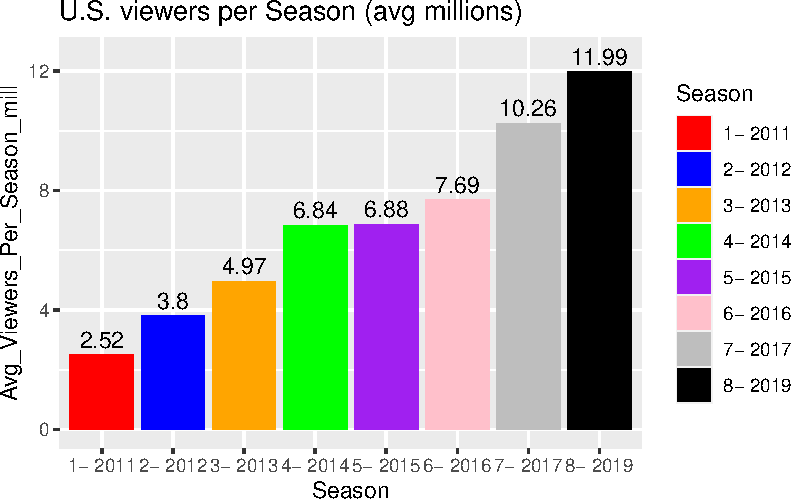
\includegraphics{RR_files/figure-pdf/unnamed-chunk-2-1.pdf}

}

\end{figure}

\hypertarget{review-of-viewership}{%
\subsubsection{\texorpdfstring{\textbf{Review of
Viewership}}{Review of Viewership}}\label{review-of-viewership}}

From the graph above, we can see a constant increase in viewership after
each season. Between when the first season was aired in 2011 and when
the last season was aired in 2019, there has been a percentage increase
of 375.4\%. Some interesting insight shows that the percentage change in
viewings between 2011 and 2012 is the highest among all the years,
indicating a significant increase in viewership in that year. Which
shows that after people realized how nice the series was, more people
got interested and decided to be a part of it. Meanwhile, the percentage
change in viewings between 2014 and 2015 is the lowest, suggesting
nothing major really happened in season 4. The overall trend shows an
increase in viewings over time, with some fluctuations in growth rate.

\hypertarget{conclusion}{%
\subsubsection{\texorpdfstring{\textbf{Conclusion}}{Conclusion}}\label{conclusion}}



\end{document}
